


\section{Auswertung}
\label{sec:auswertung}
In diesem Kapitel werden die aufgenommenen Messwerte ausgewertet.
Es werden die Rotationswinkel für folgende Galliumarsenid-Proben bestimmt:

\begin{table}
\centering
\caption{Verwendete GaAs-Proben}
\begin{tabular}{l c c c}
\toprule
&{Probe 1}&{Probe 2}&{Probe 3}\\
&stark dotiert&schwach dotiert&hochrein\\
\midrule
L [\SI{}{\milli\metre}]&\SI{1,296}{}&\SI{1,36}{}&\SI{5,11}{}\\
N [\SI{}{\per\centi\metre\cubed}]&\SI{2,8e18}{}&\SI{1,2e18}{}&0\\
\bottomrule
\label{tab:gaasproben}
\end{tabular}
\end{table}

wobei N die Donatorenkonzentration und L die Probendicke sind.

\subsection{Magnetflussdichte am Ort der Probe}

Die Messwerte der Magnetflussdichte entlang der optischen Achse, die hier als z-Achse definiert ist, sind in \autoref{tab:magn} zu sehen.
In \autoref{fig:magn} sind diese Werte gegeneinander aufgetragen.
Der größte Wert der Magnetflussdichte beträgt:

\begin{equation}
\label{bfeldwert}
\text{B} = \SI{412}{\milli\tesla}
\end{equation}

Für die restlichen Rechnungen wird angenommen, dass die Magnetflussdichte am Ort der Probe diesem Wert entspricht.


\begin{table}
\centering
\caption{Messwerte der Magnetflussdichte B entlang der optischen Achse z}
\begin{tabular}{c c}
\toprule
{z [mm]}&{B [mT]}\\
\midrule
78	&	270	\\
80	&	327	\\
82	&	372	\\
84	&	399	\\
86	&	411	\\
88	&	412	\\
90	&	405	\\
92	&	386	\\
94	&	352	\\
96	&	297	\\
98	&	230	\\
\bottomrule
\label{tab:magn}
\end{tabular}
\end{table}


\begin{figure}
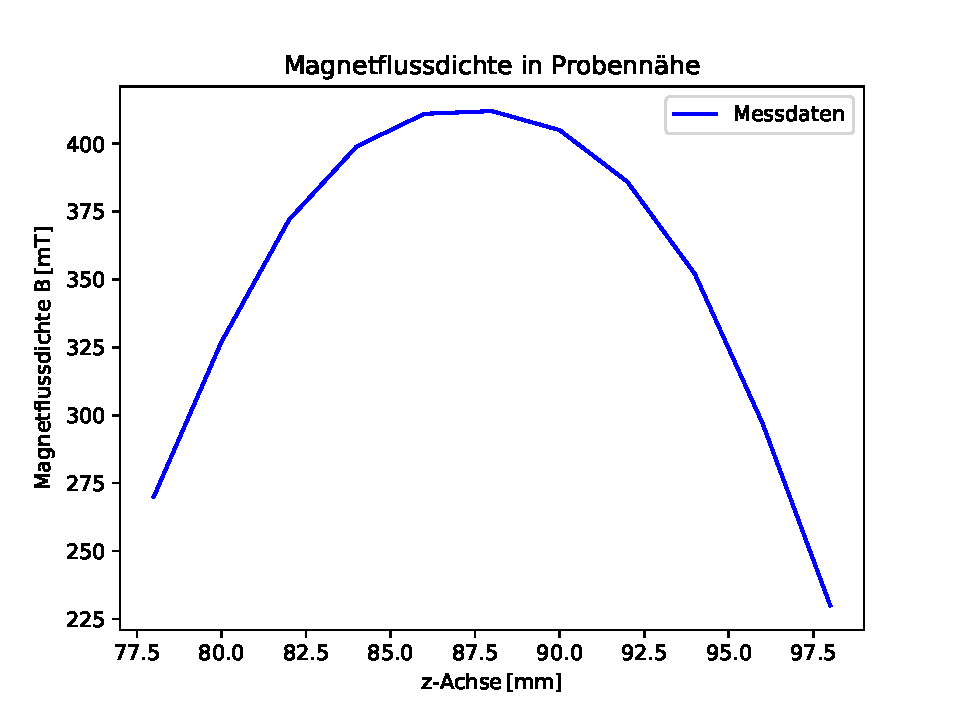
\includegraphics{content/grafiken/BFeld.pdf}
\caption{Magnetflussdichte}
\label{fig:magn}
\end{figure}




\subsection{Rotationswinkel der Faraday-Rotation}

Die gemessenen Winkel $\theta$ zur Bestimmung der Faraday-Rotation sind in \autoref{tab:farad1} zu finden.
Dabei bezeichnen $\theta_+$ und $\theta_-$ die Winkel zu unterschiedlich gepoltem Magnetfeld.


\begin{table}
\centering
\caption{Gemessene Winkel zur Faraday-Rotation}
\begin{tabular}{|l|c c|c c|c c|}
\hline
&\multicolumn{2}{c|}{Probe 1}&\multicolumn{2}{c|}{Probe 2}&\multicolumn{2}{c|}{Probe 3}\\
$\lambda$ [µm]&$\theta_+$&$\theta_-$&$\theta_+$&$\theta_-$&$\theta_+$&$\theta_-$\\
\hline
2,650&74°2'&68°57'&68°30'&60°11'&65°1'&61°13'\\
2,510&28°18'&23°38'&24°57'&11°28'&32°58'&29°6'\\
2,340&10°36'&40°35'&74°8'&68°2'&48°50'&44°30'\\
2,156&76°28'&64°3'&73°30'&66°58'&72°13'&67°21'\\
1,960&72°30'&67°4'&74°45'&68°10'&74°9'&68°36'\\
1,720&160°19'&150°45'&79°5'&72°33'&80°32'&72°45'\\
1,450&81°31'&73°45'&79°53'&74°44'&83°47'&70°30'\\
1,290&81°15'&71°15'&79°12'&73°8'&82°58'&68°20'\\
1,060&84°22'&73°9'&81°50'&72°4'&88°13'&66°32'\\
\hline
\end{tabular}\label{tab:farad1}
\end{table}

Für den Faraday-Rotationswinkel $\theta$ gilt:
\begin{equation}
\theta = \frac{|\theta_+-\theta_-|}{2}
\end{equation}

Die sich damit ergebenen Rotationswinkel sind in Radiant umgerechnet und bezogen auf die jeweilige Probendicke L als $\theta_\text{KR}$ in \autoref{tab:farad2} aufgelistet.

\begin{table}
\centering
\caption{Faraday-Rotationswinkel}
\begin{tabular}{l c c c}
\toprule
&Probe 1&Probe 2&Probe 3\\
$\lambda$ [µm]&$\theta_\text{KR}$ [\SI{}{\per\metre}]&$\theta_\text{KR}$ [\SI{}{\per\metre}]&$\theta_\text{KR}$ [\SI{}{\per\metre}]\\
\midrule
2,65	&	34,22874	&	53,36515	&	6,48948	\\
2,51	&	31,42311	&	86,51785	&	6,60333	\\
2,34	&	201,89347	&	39,14158	&	7,40029	\\
2,156	&	83,60791	&	41,92212	&	8,31109	\\
1,96	&	36,58548	&	42,24296	&	9,47806	\\
1,72	&	64,41737	&	41,92212	&	13,29205	\\
1,45	&	52,29703	&	33,04576	&	22,68473	\\
1,29	&	67,33523	&	38,92769	&	24,99020	\\
1,06	&	75,52769	&	62,66930	&	37,02990	\\
\bottomrule
\end{tabular}\label{tab:farad2}
\end{table}

Die Rotationswinkel je Einheitslänge aus \autoref{tab:farad2} sind in \autoref{fig:probe1}, \autoref{fig:probe2} und \autoref{fig:probe3} gegen das Quadrat der Wellenlänge $\lambda$ aufgetragen.

\begin{figure}
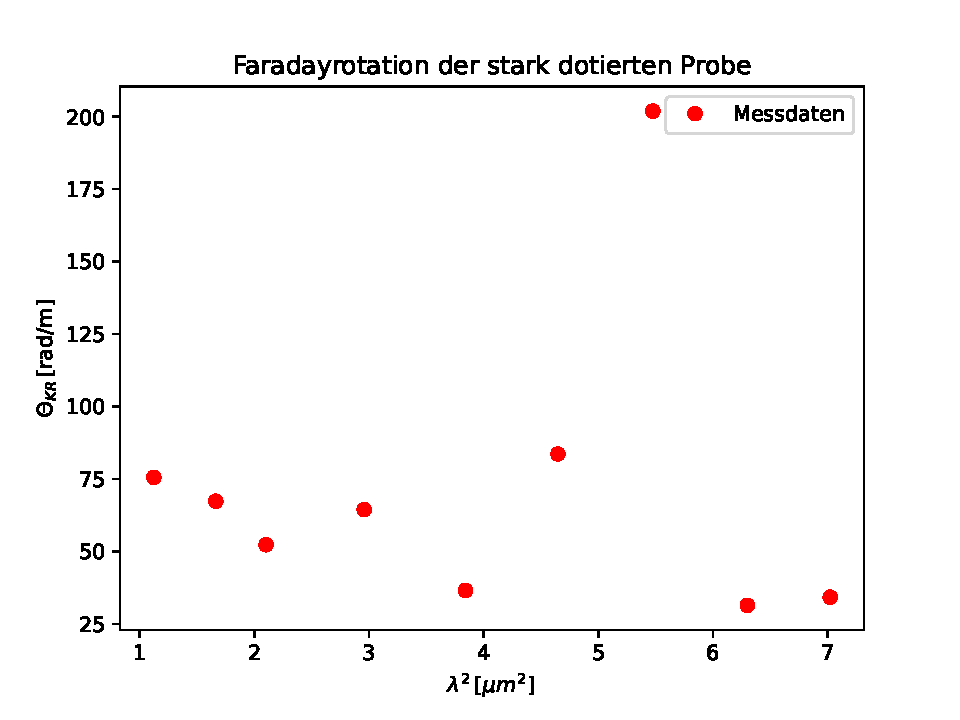
\includegraphics{content/grafiken/probe1erstes.pdf}
\caption{Rotationswinkel pro Einheitslänge der ersten Probe}
\label{fig:probe1}
\end{figure}

\begin{figure}
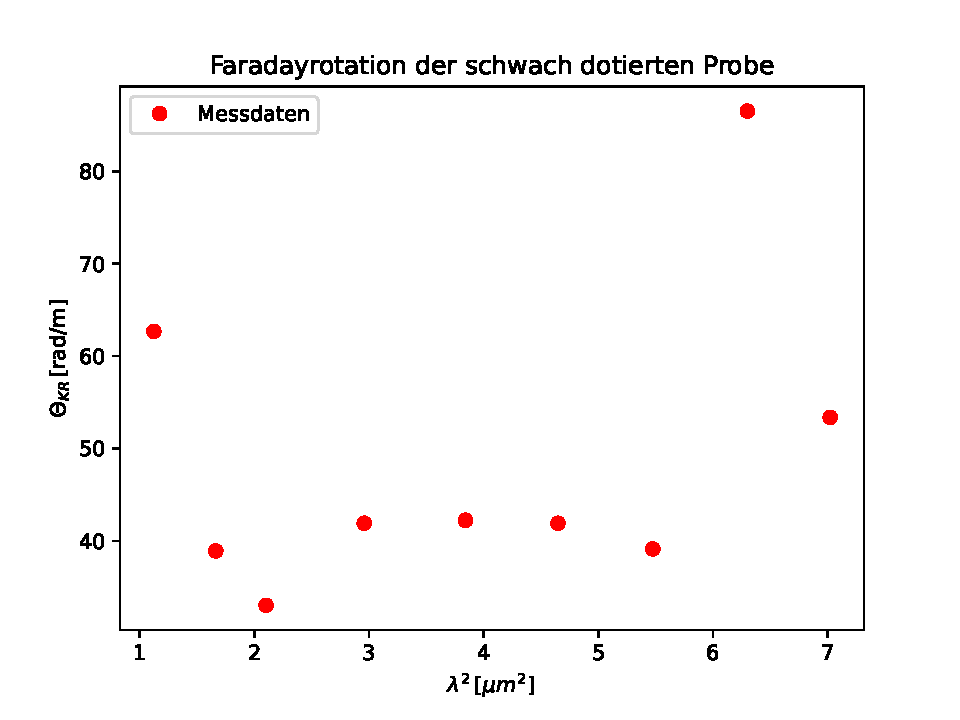
\includegraphics{content/grafiken/probe2erstes.pdf}
\caption{Rotationswinkel pro Einheitslänge der zweiten Probe}
\label{fig:probe2}
\end{figure}

\begin{figure}
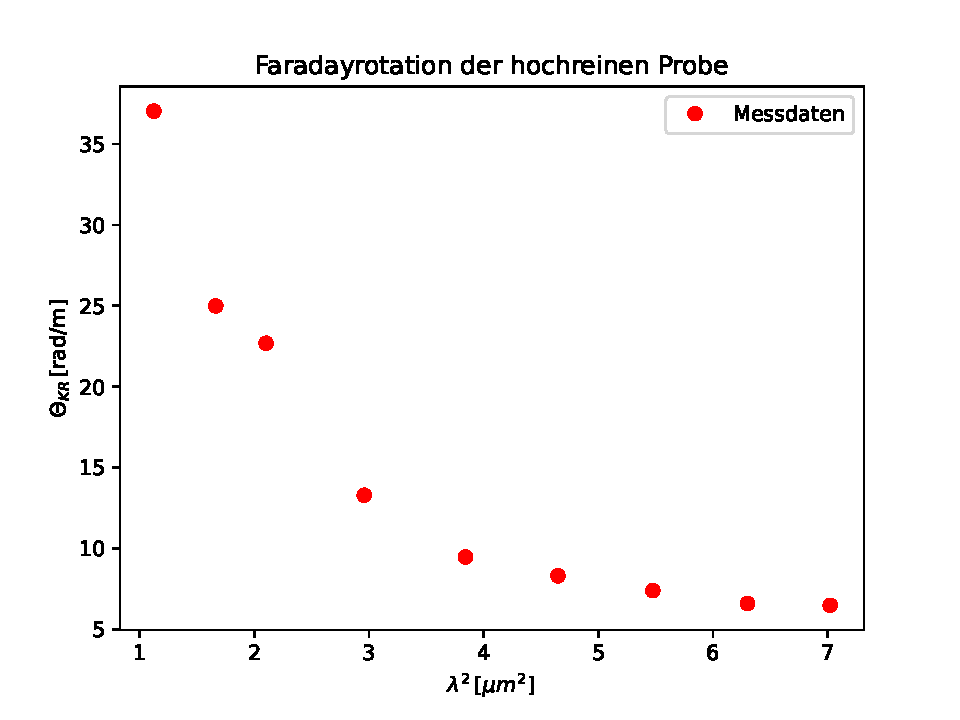
\includegraphics{content/grafiken/probe3erstes.pdf}
\caption{Rotationswinkel pro Einheitslänge der dritten Probe}
\label{fig:probe3}
\end{figure}



\clearpage


\subsection{Effektive Masse}

Um den Einfluss, den die Leitungsband-Elektronen auf den Rotationswinkel haben, zu bestimmen, wird der Rotationswinkel pro Einheitslänge der hochreinen Probe von denen der dotierten Proben abgezogen.
Die sich ergebenden Rotationswinkel $\theta_{frei}$ sind in \autoref{tab:farad3} zu sehen.
Sie sind laut \autoref{eq:thetafrei} proportional zu $\lambda^2$.
Es wird daher folgende Funktion an die Daten gefittet:
\begin{equation}
\label{eq:fit}
\theta_{frei} = a\cdot \lambda^2
\end{equation}
Für den Parameter $a$ gilt somit:
\begin{equation}
a = \frac{e_0^3NB}{8\pi^2\epsilon_0c^3(m^{\star})^2n}
\end{equation}
und daraus folgend für die effektive Masse $m^\star$ der Leitungsband-Elektronen:
\begin{equation}
m^\star = \sqrt{\frac{e_0^3NB}{8\pi^2\epsilon_0c^3an}}
\end{equation}


\begin{table}
\centering
\caption{Freie Rotationswinkel der Leitungsband-Elektronen}
\begin{tabular}{l r r}
\toprule
&Probe 1&Probe 2\\
$\lambda$ [µm]&$\theta_{frei}$ [\SI{}{\per\metre}]&$\theta_{frei}$ [\SI{}{\per\metre}]\\
\midrule
2,65	&	27,74	&	46,88	\\
2,51	&	24,82	&	79,91	\\
2,34	&	194,49	&	31,74	\\
2,156	&	75,30	&	33,61	\\
1,96	&	27,11	&	32,76	\\
1,72	&	51,13	&	28,63	\\
1,45	&	29,61	&	10,36	\\
1,29	&	42,35	&	13,94	\\
1,06	&	38,50	&	25,64	\\
\end{tabular}\label{tab:farad3}
\end{table}

Die Messdaten aus \autoref{tab:farad3} und die Fits der Funktion \autoref{eq:fit} sind für Probe 1 in \autoref{fig:probe1leit} und für Probe 2 in \autoref{fig:probe2leit} zu sehen.
Für den Parameter $a$ ergeben sich folgende Werte:
\begin{equation} \label{eq:para}
\begin{split}
a_\text{Probe1}& = \SI{12,73\pm4,20e12}{\per\metre\cubed}\\
a_\text{Probe2}& = \SI{8,39\pm1,02e12}{\per\metre\cubed}
\end{split}
\end{equation}
Daraus lässt sich die effektive Masse berechnen zu\footnote{der Brechungsindex n wurde dabei http://www.ioffe.ru/SVA/NSM/Semicond/GaAs/optic.html entnommen}:
\begin{equation} \label{eq:efmas}
\begin{split}
m^\star_\text{Probe1}& = \SI{0,085\pm0,028}{m_e}\\
m^\star_\text{Probe2}& = \SI{0,068\pm0,008}{m_e}
\end{split}
\end{equation}
Die Unsicherheiten wurden mittels Gaußscher Fehlerfortpflanzung berechnet.

\begin{figure}
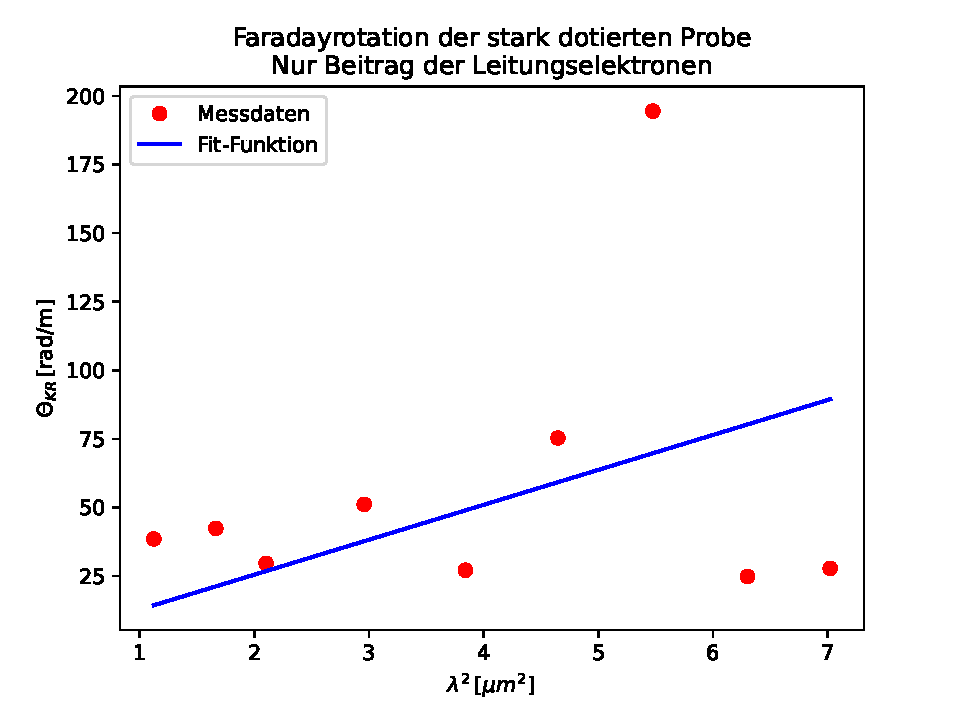
\includegraphics{content/grafiken/probe1leitungs.pdf}
\caption{Freier Faraday-Rotationswinkel für Leitungsband-Elektronen der ersten Probe mit Fit der Funktion \autoref{eq:fit}}
\label{fig:probe1leit}
\end{figure}



\begin{figure}
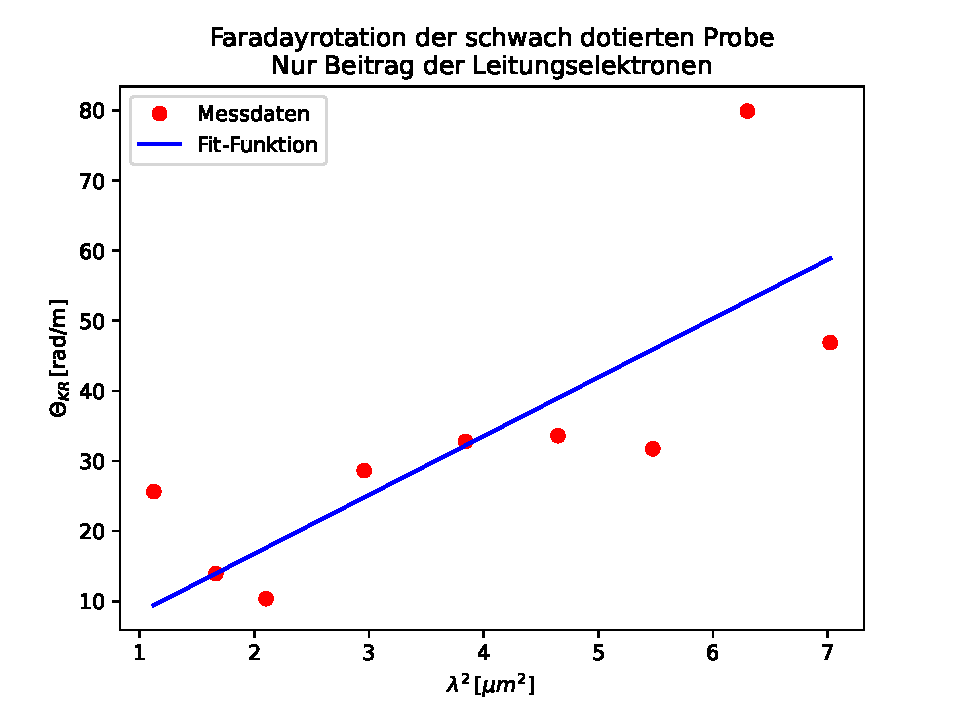
\includegraphics{content/grafiken/probe2leitungs.pdf}
\caption{Freier Faraday-Rotationswinkel für Leitungsband-Elektronen der zweiten Probe mit Fit der Funktion \autoref{eq:fit}}
\label{fig:probe2leit}
\end{figure}

























